\documentclass{bioinfo}

\usepackage[rightcaption]{sidecap} % Allows captions besides figures
%\usepackage{url} % Allows using the\url command (in NimbleGen citation)
%\usepackage{fixltx2e} % Can be used to force the order of images As-Is.

\copyrightyear{2012}
\pubyear{2012}

\newcommand{\NEW}[1]{\textcolor{red}{#1}}

\hyphenation{
microRNA
microRNAs
miRNA
miRNAs
straight-for-ward
}

\begin{document}
\firstpage{1}

\title[Visualization of cross-platform microarray data]{Pathway-based visualization of cross-platform microarray datasets}
\author[Clemens Wrzodek \textit{et~al}]{Clemens Wrzodek\,$^{1\footnote{to whom correspondence should be addressed}}$, Johannes Eichner\,$^{1}$ and Andreas Zell\,$^1$}

\address{$^{1}$Center for Bioinformatics Tuebingen (ZBIT), \\University of Tuebingen, 72076 T\"ubingen, Germany}
\history{Received on XXXXX; revised on XXXXX; accepted on XXXXX}

\editor{Associate Editor: XXXXXXX}

\maketitle

\begin{abstract}

\section{Motivation:}
Traditionally, microarrays were almost exclusively employed for the genome-wide analysis of differential gene expression. But nowadays, their scope of application has been extended to various genomic features, such as microRNAs, proteins, and DNA methylation.
Most available methods for the visualization of these datasets are focused on individual platforms and are not capable of integratively visualizing multiple microarray datasets from cross-platform studies.
Above all, there is a demand for methods that can visualize genomic features that are not directly linked to protein-coding genes, such as regulatory RNAs (e.g., microRNAs) and epigenetic alterations (e.g., DNA methylation), in a pathway-centered manner.

\section{Results:}
We present a novel pathway-based visualization method that is especially suitable for the visualization of high-throughput datasets from multiple different microarray platforms which were employed for the analysis of diverse genomic features in the same set of biological samples.
The proposed methodology includes concepts for linking DNA methylation and microRNA expression datasets to canonical signaling and metabolic pathways.
We further point out strategies for displaying data from multiple proteins and protein modifications corresponding to the same gene. Ultimately, we show how data from four distinct platform types (mRNA, miRNA, protein, and DNA methylation arrays) can be integratively visualized in the context of canonical pathways.


\section{Availability:}
The described method is implemented as part of the InCroMAP application that is freely available at \href{http://www.cogsys.cs.uni-tuebingen.de/software/InCroMAP/}{www.cogsys.cs.uni-tuebingen.de/software/InCroMAP}.


\section{Contact:} \href{mailto:clemens.wrzodek@uni-tuebingen.de}{clemens.wrzodek@uni-tuebingen.de}
\end{abstract}


%%%%%%%%%%%%%%%%%%%%%%%%%%%
% MAPK different steps to visualization PICTURE
%%%%%%%%%%%%%%%%%%%%%%%%%%%
\begin{figure*}[t]
\centering
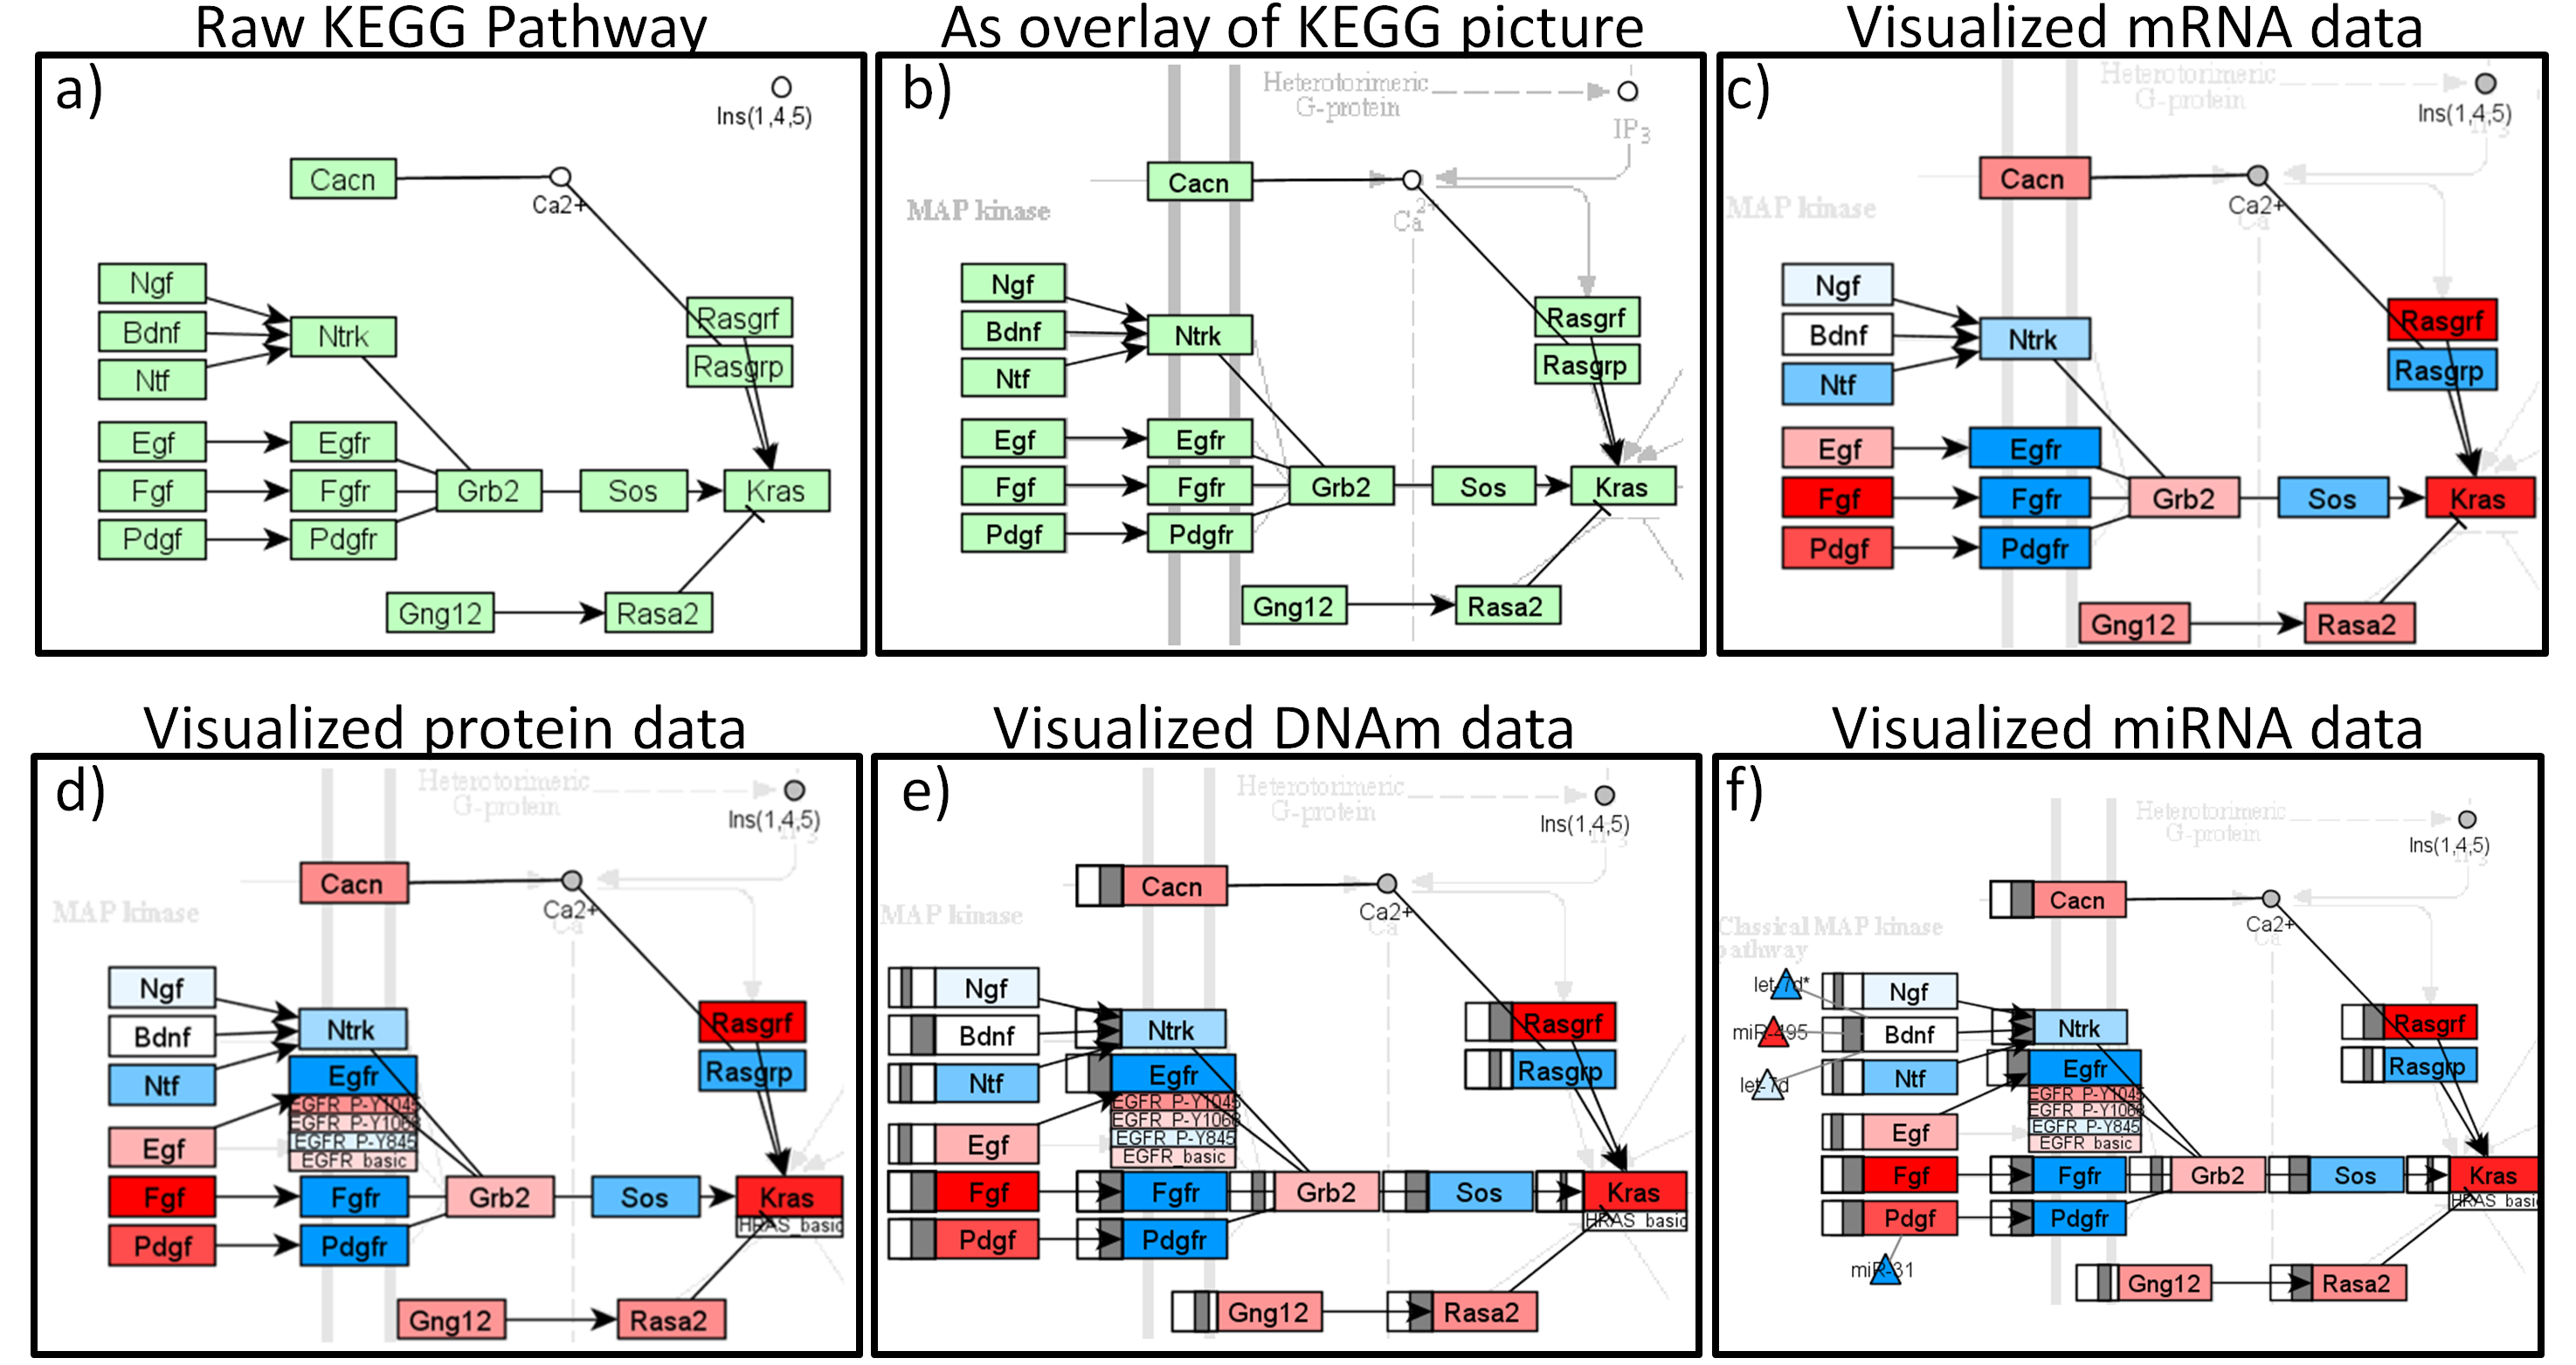
\includegraphics[width=1.0\textwidth]{WrzodekFig01.png}
\caption{These pictures show an excerpt of the KEGG `MAPK signaling' pathway. It is demonstrated how the
pathway and each of the four supported platforms are visualized in the pathway. Picture a) shows the
pathway from the KGML document visualized as a graph. b) indicates that the information content of KEGG
pathway visualizations can be improved by underlaying the original KEGG pathway picture. c) shows the
pathway overlaid with mRNA expression data, where red means upregulation, blue indicates downregulation, and
more saturated colors correspond to stronger differential expression. d) shows how protein modification datasets are
visualized in the pathway. Each box below the node \emph{Egfr} represents a different modification of the corresponding
protein and the color of the box reflects the corresponding fold-change. e) illustrates DNA
methylation peaks in promoter regions. A bar from the middle of the black box to the left represents
hypomethylation and hypermethylation is indicated by a bar to the right. The size of the bar
corresponds to the size of the maximum DNA methylation peak. f) demonstrates the visualization of
microRNA data by adding small triangles, representing microRNAs, and connecting them to their mRNA targets.
The color of the microRNA nodes refers to the corresponding fold-changes.}
\label{fig:visualization_steps}
\end{figure*}
%%%%%%%%%%%%%%%%%%%%%%%%%%%


\section{Introduction}

The first generation of microarray platforms was developed as a high-throughput technique for
profiling the transcriptome of diverse biological systems (i.e., cells, organs or organisms) under
various experimental conditions \citep{Schena1995, Golub1999}. As these traditional gene-centered
arrays were mostly limited to mRNA transcripts, the vast majority of visualization tools is focused
on mRNA datasets (e.g., Expression Profiler -- \citealp{Kapushesky2004} or KegArray --
\citealp{KEGG}). To date, a plethora of different microarray platforms are readily available. These
include gene-centered platforms which rely on current genome annotations as well as unbiased tiling
arrays which interrogate large non-repetitive regions of the genome. Diverse types of platforms have
been specifically designed for the interrogation of different genomic features, ranging from mRNA or
miRNA transcripts, through proteins or protein modifications, to relevant functional elements such
as exons, SNPs or promoters \citep{Hoheisel2006}. In addition to arrays serving for the
quantification of global gene expression on the RNA or protein level, also epigenetic modifications
such as DNA methylation can be monitored on a genome-wide level using microarray technology
\citep{Schumacher2006}.

% Motivation fuer die Entwicklung des Tools
Several tools exist for the visual inspection of datasets from individual platforms \citep[see][for
some examples]{Gehlenborg2010}. However, the current inventory of publicly available tools, that are
capable of integrating and jointly visualizing data from multiple microarray platforms, is still
very limited. Here, we introduce a method for integrated pathway-centered visualization of
datasets, generated from the same biological samples using different microarray platforms, which
monitor complementary genomic and epigenomic features.

% Pathway-basierte Visualisierung vs. Regions-basierte Visualisierung
In contrast to commonly used region-based visualization methods (e.g., the UCSC genome browser --
\citealp{UCSCBrowser}), we propose to visualize the microarray data in the context of specific
signaling or metabolic pathways, which can in many cases be more easily related to the biological
problem under study, than individual genes or genomic regions.
%
% InCroMAP vs. publizierte Pathway-basierte Visualisierungstools
In recent years, diverse tools were developed, which are specialized in pathway analysis (e.g.,
Ingenuity) or pathway visualization (e.g., Cytoscape -- \citealp{Cytoscape} or KEGG Atlas --
\citealp{KEGGAtlas}). Some of these tools offer visualizing experimental data in a pathway (e.g.,
KegArray -- \citealp{KEGG}, Pathline -- \citealp{Pathline}, GenMAPP -- \citealp{GenMAPP} or MGV -- \citealp{Symons2011}). For this
purpose, the experimental data is typically mapped to a color gradient and displayed in the
background color of the pathway nodes. GenMAPP or MGV even have capabilities to display multiple
colors in a single node (e.g., for the visualization of time-series experiments). MGV goes one step
further and offers additional features to put profile plots or heatmaps inside nodes. However, all
of these tools are not able to handle data from genomic features which have no direct reference to
the genes in a pathway (e.g., microRNAs or genomic regions). Furthermore, none of these tools offers
viable solutions that are tailored for the integration of multiple datasets obtained from
heterogeneous microarray platforms.



%\begin{methods}
\section{Methods}

% Import von Microarray-Daten in InCroMAP
% (Refs zu Ringo, MEDME, AgiMicroRna, Limma, Annotate)
Before visualization, the microarray datasets of interest have to be preprocessed and annotated
using platform-specific workflows \citep{Limma, AgiMicroRna}. These workflows usually involve (1)
the quality control of the raw data \citep{arrayQualityMetrics}, (2) the data normalization to
correct for background noise and experimental variation \citep{Lim2007}, and (3) the mapping of
probes to genes or genomic regions. After these preprocessing steps the microarray data has to be
exported in tabular format. These tables have to contain two types of columns: (1) annotation
columns, containing probe or probeset IDs (e.g., Affymetrix IDs) and database IDs of the
corresponding genes (e.g., Ensembl or Entrez IDs), and (2) data columns containing either
fold-changes and/or \emph{p}-values resulting from basic statistical analysis of the microarray
data.

% Import von Pathways in InCroMAP
The pathway data is automatically imported from KEGG \citep{KEGG}. In the KEGG PATHWAY database, each pathway map
is available for download as KGML document, which is internally converted into a graph structure
by InCroMAP. In order to overcome limitations of the KGML format, one can create an overlay
graph that shows the original KEGG pathway image in the background, which may provide the user with
additional information about cellular structure and compartmentalization.
%
% Selektierung von graphen
\NEW{Relevant pathways can be deduced by a gene-set enrichment analysis or simply by manually choosing any pathway to visualize.}
%
% Visualisierung von Microarray-Daten im Kontext von Pathways
After importing the data, the KEGG pathway nodes, which correspond to genes or gene families, can be
overlaid with fold-changes measured on mRNA or protein expression level. Furthermore, DNA
methylation changes observed in the proximal promoter regions can be visualized. In the final step,
additional nodes corresponding to miRNAs can be added to the pathway and colored according to the
expression changes measured in the underlying experiment. See Figure~\ref{fig:visualization_steps}
for an illustration of all the above-mentioned visualization steps.


%%%%%%%%%%%%%%%%%%%%%%%%%%%
% CELL CYCLE PICTURE
%%%%%%%%%%%%%%%%%%%%%%%%%%%
\begin{SCfigure*}[1][tb]
\centering
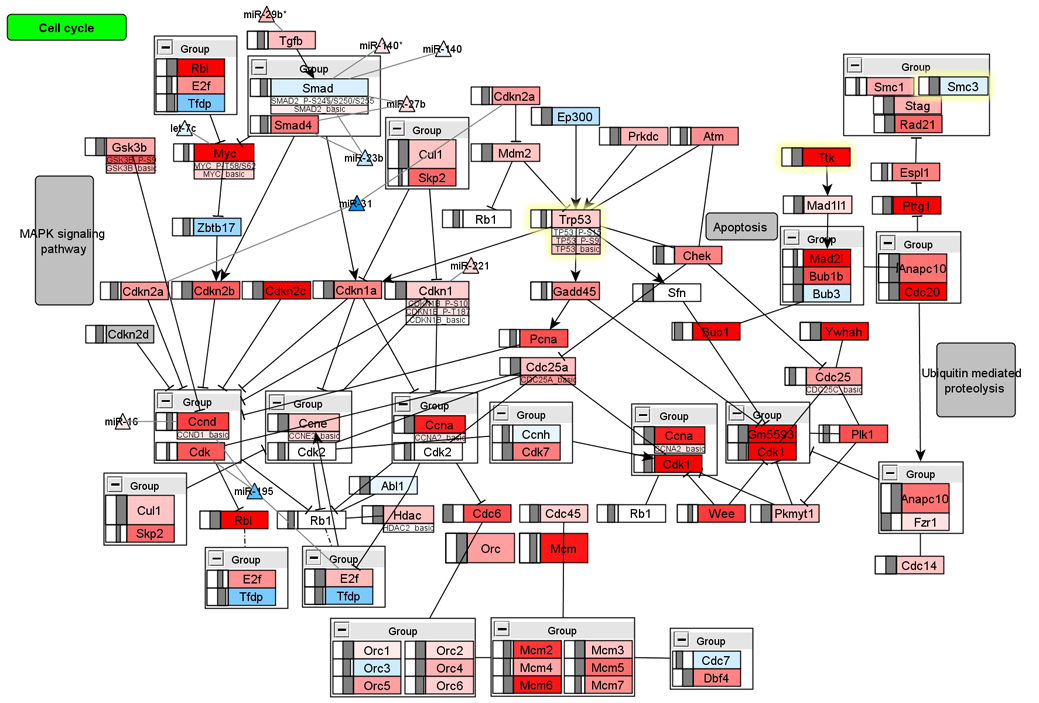
\includegraphics[width=.675\textwidth]{WrzodekFig02.png}
\caption{Integrated visualization of datasets from four different platforms in the KEGG `Cell Cycle' pathway.
%We highlighted three examples, which are mentioned below, with a light yellow color to ease finding the mentioned nodes.
In general, colors reflect fold-changes, where red means upregulated and blue means
downregulated. White indicates a fold-change of zero and darker colors correspond to stronger
differential expression. The color of each node itself reflects the mRNA fold-change, e.g., \emph{Ttk}
shows a strong upregulation and \emph{Smc3} is downregulated. Smaller boxes below nodes show the protein
and protein modification expression. For example, we visualized three different forms of TRP53: a
phosphorylation at the Serine 15 (S15) site, which shows almost no expression change, a modification
% Bitte das komma vor dem AND lassen (ein sog. "serial comma").
of the S9 site, which is upregulated, and the basic protein itself, which is also upregulated. The
black boxes left of the nodes represent the maximum DNA methylation fold-change peak. A bar to the
left indicates hypomethylation and a bar to the right hypermethylation. In our example, \emph{Ttk} shows
a strong hypermethylation.
All above mentioned genes are highlighted in yellow.
MicroRNAs are added as small triangles to the pathway and connected with
a grey edge to their mRNA targets. The color of the microRNA nodes reflects the fold-change, as
described for the mRNA nodes.}
\label{fig:cellcycle}
\end{SCfigure*}
%%%%%%%%%%%%%%%%%%%%%%%%%%%

\subsection{Pathway visualization}

The basic prerequisite for generating a pathway-based visualization is visualizing the pathway
itself. For this purpose, we are using KEGGtranslator \citep[see][]{Wrzodek2011}, which performs a
basic conversion of the KEGG KGML documents to GraphML. In short, KEGGtranslator converts all KGML entries to nodes
and all relations to edges. \NEW{Compounds are depicted by small circular nodes, genes or proteins are rectangular shaped nodes and group nodes are used to illustrate compounds or families.}
%Some basic errors are corrected automatically and appropriate shapes, colors and labels are inferred.
Then, all nodes are annotated with diverse identifiers (e.g., Entrez Gene
identifiers -- \citealp{EntrezGene}),
descriptions, and further information. The resulting document provides the basis for the
subsequently generated visualizations.

% Vorteile des Pathway-Bilds im Hintergrund
At least for some pathways, the KGML document available at KEGG does not contain all information
that is depicted in the corresponding pathway map. Thus, an overlay graph can be generated which contains the
original pathway map as a static transparent image in the background of the interactive graph plot
(see Figure~\ref{fig:visualization_steps}b). By using the given x and y coordinates together with height and width of each interactive node, it is possible
to match each node exactly on the background pathway picture. However, to allow a clear distinction between the actual pathway in the foreground and the pathway background picture, the background picture should be brightened by at least 70\,\%.
%Furthermore, this is just an optional recommended step that allows for the creation of integrated pathway plots with additional information like compartments or further descriptions.
Owing to this optional feature, additional information on
cellular structure (e.g., schematic drawings of receptors involved in cell signaling) can be maintained.



\subsection{Visualization of messenger RNA expression data}

% Darstellung von mRNA Daten
As mRNA expression data is typically available for the whole genome and thus, also for the majority
of nodes in a particular KEGG pathway, these data are displayed in the background color of the
nodes.
%
% Eingabeformat für mRNA Daten
As input, our method requires preprocessed mRNA datasets with annotation columns (e.g.,
gene identifiers) and data columns, which are referred to as \emph{observations}. In this context,
observations can be any statistical significance (e.g., \emph{p}-values) or comparative measure
(e.g., fold-changes or log-ratios).

% Mapping von mRNA Daten auf Pathway-Knoten
Next, these data have to be broken down to a single value for each pathway node, which then
determines the color of the node. As single nodes can represent multiple genes in KEGG, the
intensities measured by probes, corresponding to the same node, have to be summarized. To this end,
either the mean or median is calculated across these probes, or the probe
with the strongest or most significant signal (i.e., $\min\emph{p}\text{-}value$ or $\max|fold\text{-}change|$) is
decisive for coloring the node.
\NEW{Among others, the InCroMAP application provides all of these summarization methods.}

% Einfärbung der Knoten
To visualize fold-changes or log-ratios in the context of pathways, a color gradient ranging from
blue through white to red is used to illustrate down- and upregulation,
respectively. Non-differentially expressed genes are shown in white, and pathway nodes for which no
mRNA data is available are displayed in grey. If desired, \emph{p}-values can be shown instead of
fold-changes. For this purpose, we decided to map the negative logarithm of the \emph{p}-values to a
color gradient, which leads to a more intuitive illustration of the observed significances. See
Figure~\ref{fig:visualization_steps}c) for an example of visualized mRNA data.


\subsection{Visualization of protein expression data}

% Darstellung von Protein-Daten
Visualization of protein datasets is performed by adding small boxes below pathway nodes and
changing the color of the boxes according to the corresponding protein expression data. As state-of-the-art
experimental techniques (e.g., reverse-phase protein arrays, quantitative mass spectrometry)
facilitate the distinction between different protein modifications (e.g., phosphorylated or
acetylated forms of proteins), multiple measurements may correspond to the same gene \citep{Pirnia2009, Yates2009}.
In this particular case, the expression change observed for each individual protein form is represented
as a separate box below the corresponding node. Each of these boxes is then labeled according to the
respective protein form and colored based on the underlying expression data, as described previously
for mRNA datasets. We require protein datasets to be annotated with database identifiers referring
to proteins or genes (e.g., Entrez Gene IDs), which allows us to perform a straightforward mapping to
pathway nodes. For protein modification datasets, we further require a column, determining the
actual modification for every protein.


\subsection{Visualization of DNA methylation data}

% Darstellung von DNAm Daten
The DNA methylation (DNAm) status, observed in the proximal promoter of a gene, is graphically
represented by adding boxes to the left side of the pathway nodes. These boxes are drawn on a white
background and contain a black bar which stretches from the middle to the left, in the case of hypomethylation and from the middle to the right, to indicate hypermethylation. Instead of discriminating between hyper- and hypomethylation, one can simply visualize the amount of differential methylation. In this case, the black bar would stretch from the left border of the box to the right border.

% Berechnung des DNAm Gesamtwerts
The length of the black bar is proportional to a summary value reflecting the DNAm status of the
promoter of a certain gene. This value is by default computed from the probes in a region ranging
from -2000 bps upstream of the transcription start site to 500 bps downstream. Normally, the
value of the maximum peak found in the promoter of a gene is visualized. For peak detection,
Nimblegen proposed two algorithms which are called `Windowed Threshold Detection' and
`Second Derivative Peak Detection'. A detailed description of these methods can be found in the
user's guide of Nimblegen's SignalMap software \citep[see][]{NimblegenSignalMapUserGuide}.
In addition to those sophisticated peak detection methods, one can also approximate peaks by
using simple methods such as picking the probe with maximum differential methylation (i.e., $\max|fold-change|$).
As an alternative to visualizing peaks derived from the probe-level fold-changes one can also use a statistical
approach to estimate the differential methylation in a promoter region. For this purpose, we
propose to divide the promoter region $r$ into segments $b_1,\dots,b_n$, each containing a fixed number of probes.
For each segment a statistical test (e.g., ordinary or moderated \emph{t}-test) can be employed to detect
differential methylation between two experimental groups. An overall significance value $s$ can then be computed
from the \emph{p}-values $p(b_1),\dots,p(b_n)$ using the formula $s=\frac{1}{n}\sum\limits_{i=1}^n-\log(p(b_i))$.
This binning approach has the advantage of being sensitive to local changes in DNA methylation, as promoter segments with
significant changes in DNA methylation are highly weighted. Conversely, segments for which slight changes were observed only
contribute marginally to the overall significance score.
\NEW{InCroMAP, by default, approximates the peak by selecting the probe with maximum differential methylation. It further supports other options, such as the given formula $s$ to process \emph{p}-values and simple options that include mean, median, minimum and maximum. If multiple genes are associated to one node, all probes are placed in a single pool and the summarization method is applied. By default, this will lead to a visual representation of the maximum peak contained in any gene that is represented by a node.}

% Darstellung der DNAm Einzelwerte
The purpose of this visualization technique is giving researchers a hint if,
and how many methylation changes are present in a gene promoter.
For more details, the genomic location of individual peaks can be visualized in a DNAm profile plot
(see Figure~\ref{fig:methdetails}). To this end, the fold-changes observed for the probes
covering the promoter region of a certain gene are plotted along their genomic coordinates. This
depiction is particularly useful for comparing the DNAm profiles and peaks found for different
observations (i.e., sample groups).

% Eingabeformat f�r DNAm Daten
In order to relate the DNAm data to data from gene-centered microarrays (e.g., mRNA expression
arrays), each probe needs to be mapped to a gene. Thus, we require annotation columns containing the
chromosome and the genomic position of each probe to facilitate the mapping from probes to genes.

%%%%%%%%%%%%%%%%%%%%%%%%%%%
% Methylation Details Picture
%%%%%%%%%%%%%%%%%%%%%%%%%%%
\begin{figure}[tb]
\centering
% Add a border
\setlength\fboxsep{1pt}
\setlength\fboxrule{1pt}
\fbox{
  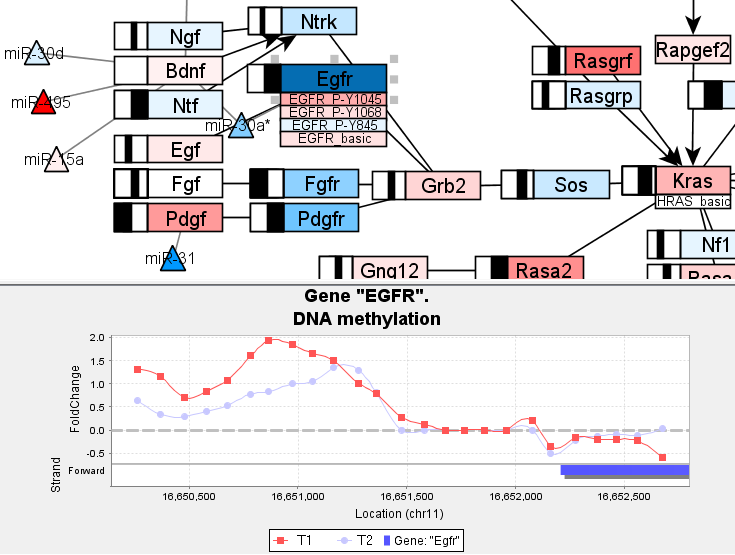
\includegraphics[width=.47\textwidth]{WrzodekFig03.png}
}
\caption{Integrated visualization of the `MAPK signaling' pathway with a detailed view of DNA methylation
in the proximal promoter of \emph{Egfr}. The black DNA methylation bar next to the \emph{Egfr} gene in the pathway
plot stretches from the middle to the right of the box, which indicates strong hypermethylation. The length
of the black bar corresponds to the height of the maximum peak of the red curve. This curve displays the probe-level
fold-changes plotted along the promoter region of \emph{Egfr}. The light blue curve shows the DNA methylation
profile of \emph{Egfr}, observed in another sample group.}
\label{fig:methdetails}
\end{figure}
%%%%%%%%%%%%%%%%%%%%%%%%%%%

\subsection{Visualization of microRNA expression data}

% Mapping von miRNA Daten auf Pathways
Visualizing microRNA (miRNA) datasets in the context of KEGG pathways is not straightforward, as
these pathways do not contain miRNAs \emph{a priori}. Therefore, in order to incorporate the data into a
pathway, a connection must be established between the miRNAs and the protein-coding genes
in the pathway. As the common mechanism of miRNAs involves the binding to complementary mRNA
transcripts \citep{Bartel2004}, we propose to link miRNAs to their known target mRNAs. These target
mRNAs can be obtained from diverse databases, which either contain experimentally verified targets
(e.g., miRecords -- \citealp{miRecords}, miRTarBase -- \citealp{miRTarBase}, TarBase --
\citealp{TarBase}) or predicted miRNA targets \citep[reviewed in][]{Alexiou2009}.
We used a union of the three mentioned experimentally verified miRNA target databases for the
figures in this publication.


% Darstellung von miRNA Daten
Based on a map containing all connections between miRNAs and their target mRNAs, the miRNAs
monitored in a specific experiment can be added to a pathway of interest as small triangular nodes,
which have outgoing edges to the pathway nodes corresponding to their target mRNAs. The triangular
miRNA nodes are colored according to their expression, as described previously for mRNA datasets.
This leads to an integrated visualization of a pathway, overlaid with miRNA and mRNA expression
data, and extended with putative miRNA-mRNA interactions. Figure~\ref{fig:visualization_steps}f)
shows an example result of the described procedure.

%\end{methods}

\section{Results and discussion}

In this work, we present a novel methodology for the combined visualization of DNA methylation data,
as well as mRNA, (phospho-) protein, and miRNA expression data in the context of canonical pathways.
This methodology involves strategies for mapping the data from heterogeneous platform types to a common
functional element, namely a gene, embedded into a pathway which regulates higher-order cellular
functions or processes. Furthermore, we propose visualization techniques which are particularly suited for
displaying quantitative data from diverse genomic features in an integrated graph plot,
which represents a metabolic or signaling pathway of interest. However, generating a joint visualization of
epigenomics, transcriptomics and proteomics data is challenging, as each data type has
its own characteristics.

% Zusammenfassung: Proteomics-Daten
For proteomics data, we propose to map basic and modified proteins to their common source gene and
draw each protein form as a separate box below the pathway node representing the source gene. Using this kind of
visualization one can, for instance, determine the activation state of a protein by comparing the color (i.e., expression state)
of the box corresponding to the basic form with the one which corresponds to the phosphorylated form.

% Zusammenfassung: Transcriptomics-Daten (mRNA (kurz), miRNA)
In brief, for most mRNA expression datasets it is sufficient to annotate the probesets with appropriate
gene identifiers, in order to link the data with the pathways of interest. For miRNA datasets this linkage
is complicated by the fact that miRNAs are normally not contained in pathways.
% miRNA discussion
A simple approach for putting miRNAs in context would be, inspecting the gene locus of the microRNAs. This approach already led to some valuable results, e.g., the detection of a strong co-regulation within the genomic DLK1 locus \citep{DLK1miRNA}. But this approach is not suitable for linking the miRNAs with genes in a pathway. Firstly, genes from neighboring loci are not generally co-regulated. Secondly, a pathway shows, for example, how a signal is processed within a certain organism. The genes in a pathway are usually functionally related or represent regulatory relationships. Hence, when adding new nodes to a pathway, the relation should also be made based on functional or regulatory relationships. MicroRNAs are known to have a regulatory function by binding to complementary mRNA transcripts \citep{Bartel2004}. These interactions are documented in public databases, which we use to extract interactions between miRNAs and their target mRNAs. Using this information, one can add the miRNAs to the pathways and connect them to the existing nodes by inserting edges to the corresponding targets.

% Zusammenfassung: Epigenomics-Daten
The probe design of DNA methylation microarrays is typically not gene-centered, but
region-based. Thus, in contrast to gene-centered arrays, the probes are not organized in
probesets which were designed specifically for the same gene. Instead, these arrays
cover specific genomic regions of interest, for instance gene promoters. The connection to protein
coding genes is usually established by defining a region around the transcription start site (TSS)
of a gene and assigning all probes in this region to the gene.
%
% Problematik bei Berechnung eines Gesamtwerts für DNAm
But visualizing the signal levels of all probes assigned to a certain gene in one pathway node would
clutter the picture and reduce the clarity of it.
Thus, we concluded that it is most important to know if there are methylation changes in a promoter and maybe also if the gene
is rather hyper- or hypomethylated. The methylation details can then be inspected manually later
(e.g., the InCroMAP application provides a detailed XY plot of the DNA methylation if one clicks on a pathway node).
Therefore, a method for the computation of a single summary value for DNA methylation probes is needed. For mRNA expression arrays, the summarization of probes corresponding to
the same transcript is usually achieved by the median polishing algorithm \citep[see][]{GCRMA} which
effectively alleviates the influence of outlier probes. However, this algorithm is only applicable under the assumption
that ideally the probe intensities are evenly distributed along transcripts.
This assumption does not hold for the DNA methylation of promoter regions, as the probe intensities are
not expected to be evenly distributed along the region. Furthermore, outlier probes, corresponding to
DNA methylation peaks, are mostly not due to probe-specific effects, but rather reflect a local change
in the DNA methylation pattern, which may be biologically meaningful. Thus, one of the summarization methods we
consider advisable is the detection and visualization of maximum peaks as it is sensitive to local changes in DNA methylation.

Alternatively, if the data is properly normalized and smoothed (i.e., probe specific effects are alleviated), one can also take the probe with maximum differential methylation to approximate the peak.
Nevertheless, every summarization method has its limitations. The maximum peak methods are definitely
less robust against probe-specific effects and the results may be inconclusive as a single positive peak may
suggest hypermethylation of a region, while the majority of the promoter is clearly hypomethylated.
%On the other hand, a mean fold-change summarization clearly suffers from the fact that localized differential methylation is averaged out. Means or medians of DNA methylation probes in a promoter region are typically close to zero.
On the other hand, if mean probe-level fold-changes are computed across larger regions, there is a higher chance that localized differential methylation is erased.

% Beispiel für Visualisierung aller Plattform-Typen in einem Pathway
An example for a KEGG pathway with visualized mRNA, miRNA, protein and DNA methylation data can be
seen in Figure~\ref{fig:cellcycle}. The visualization of multiple heterogenous datatypes can not be
performed with either a loss of information or a loss of clarity. Since these integrated pathway
visualizations should provide an overview, rather than a detailed listing of all possible
information, we tried to keep the clarity and summarize information wherever possible.

At first glance, it always seems to be desirable putting as much information as possible into the pathway. For example, it would be possible to create small XY plots of promoter regions for every gene and add these pictures as small icons below each node. Other possibilities include the creation of heatmaps or visualization of multiple timepoints with various colors in a single node.
But, especially if multiple datasets are visualized together in a pathway, it is very important to summarize things and to not overload the whole picture. The main purpose of a pathway-based visualization is not to replace all other analysis and visualization methods, but rather giving a general overview that helps researchers further analyzing their data.


\section{Implementation and availability}
The described methods are implemented in InCroMAP, a tool for integrated analysis of cross-platform microarray and Pathway data.
InCroMAP is a Java\texttrademark{} application that provides an interactive, user-friendly and easy-to-use graphical user interface (GUI), and is freely available under the LGPL version 3 license from \href{http://www.cogsys.cs.uni-tuebingen.de/software/InCroMAP/}{www.cogsys.cs.uni-tuebingen.de/software/InCroMAP}. The application can import all mentioned data types, is able to automatically download and layout KEGG pathways, and apply all described visualization methods on those pathways. The resulting graphs can be exported as JPG, GIF, TGF, GML or GraphML. Furthermore, many options are provided that control, e.g., the mapping of expression values to a continuous color gradient and allow for customization of the generated cross-platform pathway visualizations.


\section{Conclusion}

Pathway enrichment analysis is a common microarray data analysis tool to discover pathways, whose
genes show significant expression changes. In most applications, these enrichments are endpoints in
analysis workflows. There are some methods or applications that can show pictures of significantly
altered pathways and a few applications can even change node shapes or colors according to a single
expression dataset. However, not only the amount of available microarray datasets is growing
rapidly, but also the number of available platforms. At present, microarray platforms exist for
profiling diverse genomic features, as for instance mRNAs, miRNAs, proteins and promoter regions.
However, the current repertoire of analysis and especially visualization methods which are specifically designed for
the analysis of cross-platform datasets is still very limited.

Here, we present a pathway-based cross-platform microarray visualization method which
can, for example, be used to inspect relevant pathways detected by pathway enrichment analyses. Especially the
visualization of DNA methylation and miRNA datasets is a feature that can not be found in other
visualization approaches. By integratively visualizing all datatypes, it helps researchers to
discover potential relationships across multiple layers of gene regulation.
% JE: Schönes Beispiel. Habe noch die DNAm vor die miRNA gesetzt um alle Plattformen in der Kausalkette unterzubringen.
% CE: Gut gemacht, nur leider zeigt InCroMAP bei miRNAs keine DNA methylattion an...
For example, the hypomethylation of a promoter may cause the upregulation of a miRNA which may in turn
downregulate the corresponding target mRNA, whereupon a connected pathway protein could change its expression or activation state.
Such complex cascades of effects, which involve multiple levels of gene regulation can be deduced from the pathway images
generated by the here presented visualization method.

\section*{Funding}
%The research leading to these results has received funding from the Innovative Medicine Initiative Joint Undertaking (IMI JU) under grant agreement nr. 115001 (MARCAR project).
This work was supported by the Innovative Medicine Initiative Joint Undertaking (IMI JU), MARCAR project [grant number 115001].

\section*{Acknowledgement}
We gratefully acknowledge contributions from Andreas Dr\"ager and Finja B\"uchel, as well as the
whole MARCAR consortium.

%\paragraph{Funding\textcolon}
%The research leading to these results has received funding from the Innovative Medicine Initiative
%Joint Undertaking (IMI JU) under grant agreement nr. 115001 (MARCAR project).

\bibliographystyle{natbib}
%\bibliographystyle{achemnat}
%\bibliographystyle{plainnat}
%\bibliographystyle{abbrv}
%\bibliographystyle{bioinformatics}
%\bibliographystyle{plain}

%\bibliography{document}
\begin{thebibliography}{}

\bibitem[Alexiou {\em et~al.}(2009)Alexiou, Maragkakis, Papadopoulos, Reczko,
  and Hatzigeorgiou]{Alexiou2009}
Alexiou, P., Maragkakis, M., Papadopoulos, G.~L., Reczko, M., and
  Hatzigeorgiou, A.~G. (2009).
\newblock Lost in translation: an assessment and perspective for computational
  {microRNA} target identification.
\newblock {\em Bioinformatics\/}, {\bf 25}(23), 3049--3055.

\bibitem[Bartel(2004)Bartel]{Bartel2004}
Bartel, D.~P. (2004).
\newblock {MicroRNAs}: genomics, biogenesis, mechanism, and function.
\newblock {\em Cell\/}, {\bf 116}(2), 281--297.

\bibitem[Cline {\em et~al.}(2007)Cline, Smoot, Cerami, Kuchinsky, Landys,
  Workman, Christmas, Avila-Campilo, Creech, Gross, Hanspers, Isserlin, Kelley,
  Killcoyne, Lotia, Maere, Morris, Ono, Pavlovic, Pico, Vailaya, Wang, Adler,
  Conklin, Hood, Kuiper, Sander, Schmulevich, Schwikowski, Warner, Ideker, and
  Bader]{Cytoscape}
Cline, M.~S., Smoot, M., Cerami, E., Kuchinsky, A., Landys, N., Workman, C.,
  Christmas, R., Avila-Campilo, I., Creech, M., Gross, B., \emph{et al.} (2007).
\newblock Integration of biological networks and gene expression data using
  {Cytoscape}.
\newblock {\em Nat Protoc\/}, {\bf 2}(10), 2366--2382.

\bibitem[Gehlenborg {\em et~al.}(2010)Gehlenborg, O'Donoghue, Baliga, Goesmann,
  Hibbs, Kitano, Kohlbacher, Neuweger, Schneider, Tenenbaum, and
  Gavin]{Gehlenborg2010}
Gehlenborg, N., O'Donoghue, S.~I., Baliga, N.~S., Goesmann, A., Hibbs, M.~A.,
  Kitano, H., Kohlbacher, O., Neuweger, H., Schneider, R., Tenenbaum, D., and
  Gavin, A.-C. (2010).
\newblock Visualization of omics data for systems biology.
\newblock {\em Nat Methods\/}, {\bf 7}(3 Suppl), S56--S68.

\bibitem[Golub {\em et~al.}(1999)Golub, Slonim, Tamayo, Huard, Gaasenbeek,
  Mesirov, Coller, Loh, Downing, Caligiuri, Bloomfield, and Lander]{Golub1999}
Golub, T.~R., Slonim, D.~K., Tamayo, P., Huard, C., Gaasenbeek, M., Mesirov,
  J.~P., Coller, H., Loh, M.~L., Downing, J.~R., Caligiuri, M.~A., Bloomfield,
  C.~D., and Lander, E.~S. (1999).
\newblock Molecular classification of cancer: class discovery and class
  prediction by gene expression monitoring.
\newblock {\em Science\/}, {\bf 286}(5439), 531--537.

\bibitem[Hoheisel(2006)Hoheisel]{Hoheisel2006}
Hoheisel, J.~D. (2006).
\newblock Microarray technology: beyond transcript profiling and genotype
  analysis.
\newblock {\em Nat Rev Genet\/}, {\bf 7}(3), 200--210.

\bibitem[Hsu {\em et~al.}(2011)Hsu, Lin, Wu, Liang, Huang, Chan, Tsai, Chen,
  Lee, Chiu, Chien, Wu, Huang, Tsou, and Huang]{miRTarBase}
Hsu, S.~D., Lin, F.~M., Wu, W.~Y., Liang, C., Huang, W.~C., Chan, W.~L., Tsai,
  W.~T., Chen, G.~Z., Lee, C.~J., Chiu, C.~M., Chien, C.~H., Wu, M.~C., Huang,
  C.~Y., Tsou, A.~P., and Huang, H.~D. (2011).
\newblock {miRTarBase: a database curates experimentally validated
  microRNA-target interactions}.
\newblock {\em Nucleic Acids Res\/}, {\bf 39}(Database issue), D163--9.

\bibitem[Kanehisa {\em et~al.}(2006)Kanehisa, Goto, Hattori, Aoki-Kinoshita,
  Itoh, Kawashima, Katayama, Araki, and Hirakawa]{KEGG}
Kanehisa, M., Goto, S., Hattori, M., Aoki-Kinoshita, K.~F., Itoh, M.,
  Kawashima, S., Katayama, T., Araki, M., and Hirakawa, M. (2006).
\newblock From genomics to chemical genomics: new developments in {KEGG}.
\newblock {\em Nucleic Acids Res\/}, {\bf 34}(Database issue), D354--D357.

\bibitem[Kapushesky {\em et~al.}(2004)Kapushesky, Kemmeren, Culhane, Durinck,
  Ihmels, K�rner, Kull, Torrente, Sarkans, Vilo, and Brazma]{Kapushesky2004}
Kapushesky, M., Kemmeren, P., Culhane, A.~C., Durinck, S., Ihmels, J., K�rner,
  C., Kull, M., Torrente, A., Sarkans, U., Vilo, J., and Brazma, A. (2004).
\newblock {Expression Profiler}: next generation--an online platform for
  analysis of microarray data.
\newblock {\em Nucleic Acids Res\/}, {\bf 32}(Web Server issue), W465--W470.

\bibitem[Kauffmann {\em et~al.}(2009)Kauffmann, Gentleman, and
  Huber]{arrayQualityMetrics}
Kauffmann, A., Gentleman, R., and Huber, W. (2009).
\newblock {arrayQualityMetrics}--a bioconductor package for quality assessment
  of microarray data.
\newblock {\em Bioinformatics\/}, {\bf 25}(3), 415--416.

\bibitem[Kent {\em et~al.}(2002)Kent, Sugnet, Furey, Roskin, Pringle, Zahler,
  and Haussler]{UCSCBrowser}
Kent, W.~J., Sugnet, C.~W., Furey, T.~S., Roskin, K.~M., Pringle, T.~H.,
  Zahler, A.~M., and Haussler, D. (2002).
\newblock The human genome browser at {UCSC}.
\newblock {\em Genome Res\/}, {\bf 12}(6), 996--1006.

\bibitem[Lim {\em et~al.}(2007)Lim, Wang, Lefebvre, and Califano]{Lim2007}
Lim, W.~K., Wang, K., Lefebvre, C., and Califano, A. (2007).
\newblock Comparative analysis of microarray normalization procedures: effects
  on reverse engineering gene networks.
\newblock {\em Bioinformatics\/}, {\bf 23}(13), i282--i288.

\bibitem[L\'{o}pez-Romero(2011)L\'{o}pez-Romero]{AgiMicroRna}
L\'{o}pez-Romero, P. (2011).
\newblock Pre-processing and differential expression analysis of {Agilent
  microRNA } arrays using the {AgiMicroRna Bioconductor} library.
\newblock {\em BMC Genomics\/}, {\bf 12}, 64.

\bibitem[Luk {\em et~al.}(2011)Luk, Burchard, Zhang, Liu, Wong, Shek, Lee, Fan,
  Poon, Ivanovska, Philippar, Cleary, Buser, Shaw, Lee, Tenen, Dai, and
  Mao]{DLK1miRNA}
Luk, J.~M., Burchard, J., Zhang, C., Liu, A.~M., Wong, K.~F., Shek, F.~H., Lee,
  N.~P., Fan, S.~T., Poon, R.~T., Ivanovska, I., Philippar, U. \emph{et al.}
  (2011).
\newblock {DLK1-DIO3 genomic imprinted microRNA cluster at 14q32.2 defines a
  stemlike subtype of hepatocellular carcinoma associated with poor survival.}
\newblock {\em J Biol Chem\/}, {\bf 286}(35), 30706--30713.

\bibitem[Maglott {\em et~al.}(2005)Maglott, Ostell, Pruitt, and
  Tatusova]{EntrezGene}
Maglott, D., Ostell, J., Pruitt, K.~D., and Tatusova, T. (2005).
\newblock {Entrez Gene}: gene-centered information at {NCBI}.
\newblock {\em Nucleic Acids Res\/}, {\bf 33}(Database issue), D54--D58.

\bibitem[Meyer {\em et~al.}(2010)Meyer, Wong, Styczynski, Munzner, and
  Pfister]{Pathline}
Meyer, M., Wong, B., Styczynski, M., Munzner, T., and Pfister, H. (2010).
\newblock {Pathline: A Tool For Comparative Functional Genomics}.
\newblock {\em Computer Graphics Forum (Proc. EuroVis 2010)\/}, {\bf 29}(3),
  1043--1052.

\bibitem[{NimbleGen Systems Inc.}(2006){NimbleGen Systems
  Inc.}]{NimblegenSignalMapUserGuide}
{NimbleGen Systems Inc.} (2006).
\newblock {SignalMap User's Guide}.
\newblock Available from {NimbleGen} at
  \href{http://www.nimblegen.com/products/lit/signalmap1.9usersguide.pdf}{www.nimblegen.com/products/lit/signalmap1.9usersguide.pdf}.
  Accessed 2012 Mar 22.

\bibitem[Okuda {\em et~al.}(2008)Okuda, Yamada, Hamajima, Itoh, Katayama, Bork,
  Goto, and Kanehisa]{KEGGAtlas}
Okuda, S., Yamada, T., Hamajima, M., Itoh, M., Katayama, T., Bork, P., Goto,
  S., and Kanehisa, M. (2008).
\newblock {KEGG Atlas} mapping for global analysis of metabolic pathways.
\newblock {\em Nucleic Acids Res\/}, {\bf 36}(Web Server issue), W423--W426.

\bibitem[Papadopoulos {\em et~al.}(2009)Papadopoulos, Reczko, Simossis,
  Sethupathy, and Hatzigeorgiou]{TarBase}
Papadopoulos, G.~L., Reczko, M., Simossis, V.~A., Sethupathy, P., and
  Hatzigeorgiou, A.~G. (2009).
\newblock The database of experimentally supported targets: a functional update
  of {TarBase}.
\newblock {\em Nucleic Acids Res\/}, {\bf 37}(Database issue), D155--8.

\bibitem[Pirnia {\em et~al.}(2009)Pirnia, Pawlak, Thallinger, Gierke, Templin,
  Kappeler, Betticher, Gloor, and Borner]{Pirnia2009}
Pirnia, F., Pawlak, M., Thallinger, G.~G., Gierke, B., Templin, M.~F.,
  Kappeler, A., Betticher, D.~C., Gloor, B., and Borner, M.~M. (2009).
\newblock Novel functional profiling approach combining reverse phase protein
  microarrays and human {3-D} ex vivo tissue cultures: expression of
  apoptosis-related proteins in human colon cancer.
\newblock {\em Proteomics\/}, {\bf 9}(13), 3535--3548.

\bibitem[Salomonis {\em et~al.}(2007)Salomonis, Hanspers, Zambon, Vranizan,
  Lawlor, Dahlquist, Doniger, Stuart, Conklin, and Pico]{GenMAPP}
Salomonis, N., Hanspers, K., Zambon, A.~C., Vranizan, K., Lawlor, S.~C.,
  Dahlquist, K.~D., Doniger, S.~W., Stuart, J., Conklin, B.~R., and Pico, A.~R.
  (2007).
\newblock {GenMAPP} 2: new features and resources for pathway analysis.
\newblock {\em BMC Bioinformatics\/}, {\bf 8}, 217.

\bibitem[Schena {\em et~al.}(1995)Schena, Shalon, Davis, and Brown]{Schena1995}
Schena, M., Shalon, D., Davis, R.~W., and Brown, P.~O. (1995).
\newblock Quantitative monitoring of gene expression patterns with a
  complementary {DNA} microarray.
\newblock {\em Science\/}, {\bf 270}(5235), 467--470.

\bibitem[Schumacher {\em et~al.}(2006)Schumacher, Kapranov, Kaminsky, Flanagan,
  Assadzadeh, Yau, Virtanen, Winegarden, Cheng, Gingeras, and
  Petronis]{Schumacher2006}
Schumacher, A., Kapranov, P., Kaminsky, Z., Flanagan, J., Assadzadeh, A., Yau,
  P., Virtanen, C., Winegarden, N., Cheng, J., Gingeras, T., and Petronis, A.
  (2006).
\newblock Microarray-based {DNA} methylation profiling: technology and
  applications.
\newblock {\em Nucleic Acids Res\/}, {\bf 34}(2), 528--542.

\bibitem[Smyth(2004)Smyth]{Limma}
Smyth, G.~K. (2004).
\newblock Linear models and empirical bayes methods for assessing differential
  expression in microarray experiments.
\newblock {\em Stat Appl Genet Mol Biol\/}, {\bf 3}, Article3.

\bibitem[Symons and Nieselt(2011)Symons and Nieselt]{Symons2011}
Symons, S. and Nieselt, K. (2011).
\newblock {MGV}: a generic graph viewer for comparative omics data.
\newblock {\em Bioinformatics\/}, {\bf 27}(16), 2248--2255.

\bibitem[Wrzodek {\em et~al.}(2011)Wrzodek, Dr\"ager, and Zell]{Wrzodek2011}
Wrzodek, C., Dr\"ager, A., and Zell, A. (2011).
\newblock {KEGGtranslator: visualizing and converting the KEGG PATHWAY database
  to various formats}.
\newblock {\em Bioinformatics\/}, {\bf 27}(16), 2314--2315.

\bibitem[Wu and Irizarry(2005)Wu and Irizarry]{GCRMA}
Wu, Z. and Irizarry, R.~A. (2005).
\newblock Stochastic models inspired by hybridization theory for short
  oligonucleotide arrays.
\newblock {\em J Comput Biol\/}, {\bf 12}(6), 882--893.

\bibitem[Xiao {\em et~al.}(2009)Xiao, Zuo, Cai, Kang, Gao, and Li]{miRecords}
Xiao, F., Zuo, Z., Cai, G., Kang, S., Gao, X., and Li, T. (2009).
\newblock {miRecords: an integrated resource for microRNA-target interactions}.
\newblock {\em Nucleic Acids Res\/}, {\bf 37}(Database issue), D105--10.

\bibitem[Yates {\em et~al.}(2009)Yates, Ruse, and Nakorchevsky]{Yates2009}
Yates, J.~R., Ruse, C.~I., and Nakorchevsky, A. (2009).
\newblock Proteomics by mass spectrometry: approaches, advances, and
  applications.
\newblock {\em Annu Rev Biomed Eng\/}, {\bf 11}, 49--79.

\end{thebibliography}


\end{document}
